% Standalone figure for the Statistical Mechanics notes.
% Unary P--T diagrams with two solid polymorphs alpha and beta.
% (a) alpha/beta line ends on the melting curve: triple point alpha+beta+L.
% (b) alpha/beta line ends on the sublimation curve: triple point alpha+beta+V,
%     with the metastable triple point alpha+L+V inside the beta field.
% Build: pdflatex unary-polymorph.tex  (or run build.sh in this folder)
\documentclass[11pt,tikz,border=2pt]{standalone}
\usepackage{amsmath,amssymb}
\usetikzlibrary{arrows.meta, positioning}
\begin{document}
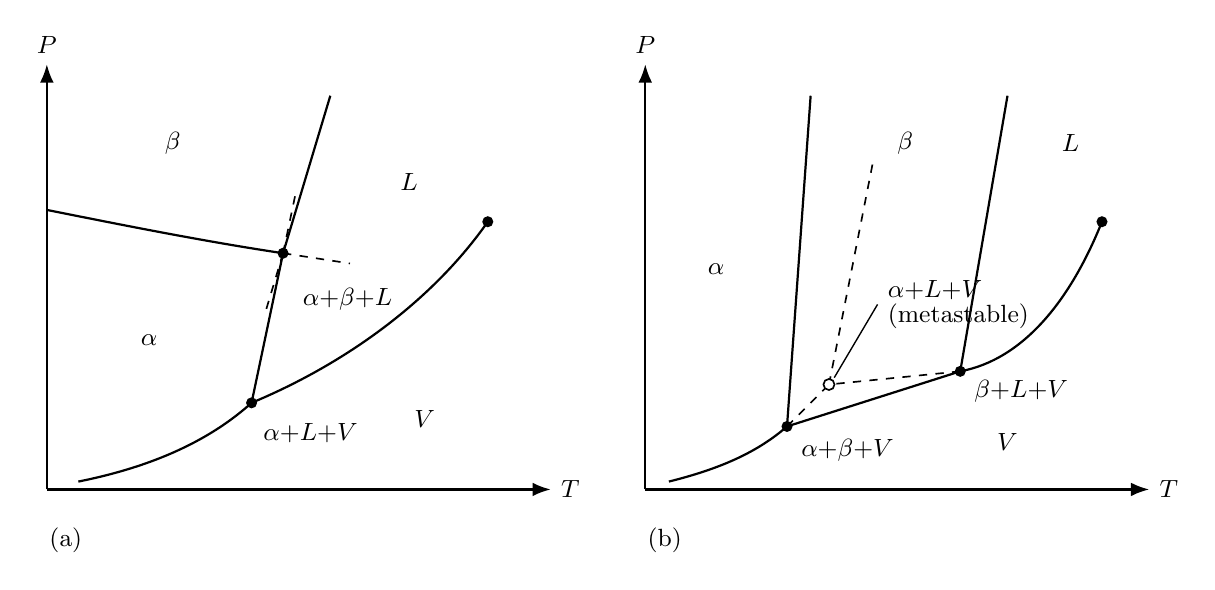
\begin{tikzpicture}[font=\small, >=Latex, line width=0.8pt]
% ------------------------------------------------------------ (a)
\begin{scope}
    \draw[->] (0,0) -- (6.4,0) node[right] {$T$};
    \draw[->] (0,0) -- (0,5.4) node[above] {$P$};
    \node[anchor=north west] at (-0.1,-0.35) {(a)};
    % alpha--vapor (sublimation)
    \draw (0.4,0.1) .. controls (1.4,0.3) and (2.1,0.65) .. (2.6,1.1);
    % liquid--vapor, ending at the critical point
    \draw (2.6,1.1) .. controls (3.8,1.6) and (4.9,2.4) .. (5.6,3.4);
    \fill (5.6,3.4) circle (2pt);
    % alpha--liquid (melting) up to the alpha+beta+L point
    \draw (2.6,1.1) -- (3.0,3.0);
    % beta--liquid
    \draw (3.0,3.0) -- (3.6,5.0);
    % alpha/beta transition line
    \draw (3.0,3.0) .. controls (2.0,3.15) and (1.0,3.35) .. (0,3.55);
    % metastable extensions beyond alpha+beta+L
    \draw[dashed, line width=0.6pt] (3.0,3.0) -- ++(0.17,0.81);   % alpha--L into beta
    \draw[dashed, line width=0.6pt] (3.0,3.0) -- ++(0.85,-0.13);  % alpha/beta into L
    \draw[dashed, line width=0.6pt] (3.0,3.0) -- ++(-0.24,-0.8);  % beta--L into alpha
    % triple points
    \fill (2.6,1.1) circle (2pt);
    \fill (3.0,3.0) circle (2pt);
    \node[right] at (2.62,0.72) {$\alpha{+}L{+}V$};
    \node[right] at (3.12,2.42) {$\alpha{+}\beta{+}L$};
    % phase labels
    \node at (1.3,1.9) {$\alpha$};
    \node at (1.6,4.4) {$\beta$};
    \node at (4.6,3.9) {$L$};
    \node at (4.8,0.9) {$V$};
\end{scope}
% ------------------------------------------------------------ (b)
\begin{scope}[xshift=7.6cm]
    \draw[->] (0,0) -- (6.4,0) node[right] {$T$};
    \draw[->] (0,0) -- (0,5.4) node[above] {$P$};
    \node[anchor=north west] at (-0.1,-0.35) {(b)};
    % alpha--vapor (sublimation) up to the alpha+beta+V point
    \draw (0.3,0.1) .. controls (0.9,0.25) and (1.4,0.45) .. (1.8,0.8);
    % beta--vapor
    \draw (1.8,0.8) -- (4.0,1.5);
    % liquid--vapor, ending at the critical point
    \draw (4.0,1.5) .. controls (4.8,1.65) and (5.4,2.4) .. (5.8,3.4);
    \fill (5.8,3.4) circle (2pt);
    % alpha/beta transition line
    \draw (1.8,0.8) .. controls (1.9,2.2) and (2.0,3.6) .. (2.1,5.0);
    % beta--liquid (melting)
    \draw (4.0,1.5) -- (4.6,5.0);
    % metastable alpha--vapor and liquid--vapor meet at alpha+L+V
    \draw[dashed, line width=0.6pt] (1.8,0.8) -- (2.333,1.333);
    \draw[dashed, line width=0.6pt] (4.0,1.5) -- (2.333,1.333);
    % metastable alpha--liquid (melting of alpha) inside the beta field
    \draw[dashed, line width=0.6pt] (2.333,1.333) -- (2.9,4.2);
    % triple points
    \fill (1.8,0.8) circle (2pt);
    \fill (4.0,1.5) circle (2pt);
    \filldraw[fill=white, line width=0.6pt] (2.333,1.333) circle (2pt);
    \node[right] at (1.85,0.5) {$\alpha{+}\beta{+}V$};
    \node[right] at (4.05,1.25) {$\beta{+}L{+}V$};
    \node[align=left, right] at (2.95,2.35) {$\alpha{+}L{+}V$\\[-2pt](metastable)};
    \draw[line width=0.5pt] (2.95,2.35) -- (2.40,1.42);
    % phase labels
    \node at (0.9,2.8) {$\alpha$};
    \node at (3.3,4.4) {$\beta$};
    \node at (5.4,4.4) {$L$};
    \node at (4.6,0.6) {$V$};
\end{scope}
\end{tikzpicture}
\end{document}
